\mbox{$\displaystyle +\,$\,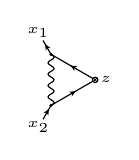
\begin{tikzpicture}[x=0.340cm, y=0.340cm, line width=0.420pt, baseline={([yshift=-0.6ex]0,0)}]
  \draw (1.100,0.000) -- (-0.550,0.953);
  \fill (0.172,0.536) -- (0.327,0.328) -- (0.311,0.455) -- (0.429,0.505) -- cycle;
  \draw (-0.550,-0.953) -- (1.100,0.000);
  \fill (0.378,-0.417) -- (0.121,-0.448) -- (0.239,-0.497) -- (0.223,-0.624) -- cycle;
  \draw plot[smooth, tension=0.7] coordinates {(-0.550,0.953) (-0.469,0.900) (-0.436,0.847) (-0.469,0.794) (-0.550,0.741) (-0.631,0.688) (-0.664,0.635) (-0.631,0.582) (-0.550,0.529) (-0.469,0.476) (-0.436,0.423) (-0.469,0.370) (-0.550,0.318) (-0.631,0.265) (-0.664,0.212) (-0.631,0.159) (-0.550,0.106) (-0.469,0.053) (-0.436,0.000) (-0.469,-0.053) (-0.550,-0.106) (-0.631,-0.159) (-0.664,-0.212) (-0.631,-0.265) (-0.550,-0.318) (-0.469,-0.370) (-0.436,-0.423) (-0.469,-0.476) (-0.550,-0.529) (-0.631,-0.582) (-0.664,-0.635) (-0.631,-0.688) (-0.550,-0.741) (-0.469,-0.794) (-0.436,-0.847) (-0.469,-0.900) (-0.550,-0.953)};
  \draw (-0.550,0.953) -- (-0.850,1.472);
  \fill (-0.775,1.342) -- (-0.744,1.084) -- (-0.694,1.202) -- (-0.567,1.186) -- cycle;
  \draw (-0.550,-0.953) -- (-0.850,-1.472);
  \fill (-0.625,-1.083) -- (-0.833,-1.239) -- (-0.706,-1.223) -- (-0.656,-1.341) -- cycle;
  \draw[fill=white] (1.100,0.000) circle (0.100);
  \draw[line width=0.298pt] (1.170,0.070) -- (1.030,-0.070) (1.170,-0.070) -- (1.030,0.070);
  \fill (-0.550,0.953) circle (0.064);
  \fill (-0.550,-0.953) circle (0.064);
  \node[font=\tiny, inner sep=0pt, anchor=180] at (1.290,0.000) {$z$};
  \node[font=\tiny, inner sep=0pt, anchor=300] at (-0.895,1.550) {$x_{1}$};
  \node[font=\tiny, inner sep=0pt, anchor=60] at (-0.895,-1.550) {$x_{2}$};
\end{tikzpicture}}
\diagramgap
\mbox{$\displaystyle -\,$\,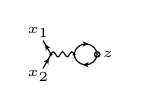
\begin{tikzpicture}[x=0.340cm, y=0.340cm, line width=0.420pt, baseline={([yshift=-0.6ex]0,0)}]
  \draw (0.287,0.000) arc[start angle=173.974, end angle=6.026, radius=0.434];
  \fill (0.838,0.388) -- (0.599,0.490) -- (0.677,0.388) -- (0.599,0.286) -- cycle;
  \draw (1.150,0.000) arc[start angle=353.974, end angle=186.026, radius=0.434];
  \fill (0.599,-0.388) -- (0.838,-0.490) -- (0.761,-0.388) -- (0.838,-0.286) -- cycle;
  \draw plot[smooth, tension=0.7] coordinates {(-0.575,0.000) (-0.532,0.066) (-0.489,0.093) (-0.446,0.066) (-0.403,0.000) (-0.359,-0.066) (-0.316,-0.093) (-0.273,-0.066) (-0.230,0.000) (-0.187,0.066) (-0.144,0.093) (-0.101,0.066) (-0.058,0.000) (-0.014,-0.066) (0.029,-0.093) (0.072,-0.066) (0.115,0.000) (0.158,0.066) (0.201,0.093) (0.244,0.066) (0.287,0.000)};
  \draw (-0.575,0.000) -- (-0.875,0.520);
  \fill (-0.800,0.389) -- (-0.769,0.131) -- (-0.719,0.250) -- (-0.592,0.233) -- cycle;
  \draw (-0.575,0.000) -- (-0.875,-0.520);
  \fill (-0.650,-0.130) -- (-0.858,-0.286) -- (-0.731,-0.270) -- (-0.681,-0.388) -- cycle;
  \draw[fill=white] (1.150,0.000) circle (0.100);
  \draw[line width=0.298pt] (1.220,0.070) -- (1.080,-0.070) (1.220,-0.070) -- (1.080,0.070);
  \fill (-0.575,0.000) circle (0.064);
  \fill (0.287,0.000) circle (0.064);
  \node[font=\tiny, inner sep=0pt, anchor=180] at (1.340,0.000) {$z$};
  \node[font=\tiny, inner sep=0pt, anchor=300] at (-0.920,0.598) {$x_{1}$};
  \node[font=\tiny, inner sep=0pt, anchor=60] at (-0.920,-0.598) {$x_{2}$};
\end{tikzpicture}}
